\documentclass{standalone}
\usepackage{tikz}
\usepackage{pgfplots}
\pgfplotsset{compat=newest}
\usepackage{amsmath}
\usepackage[american]{circuitikz}
\usepackage{cmbright}

\definecolor{myred}{RGB}{170,0,0}
\definecolor{myblue}{RGB}{0,0,220}
\definecolor{mygreen}{RGB}{0,150,0}
\definecolor{myorange}{RGB}{255,127,0}
\definecolor{mybrown}{RGB}{150,75,0}

\begin{document}
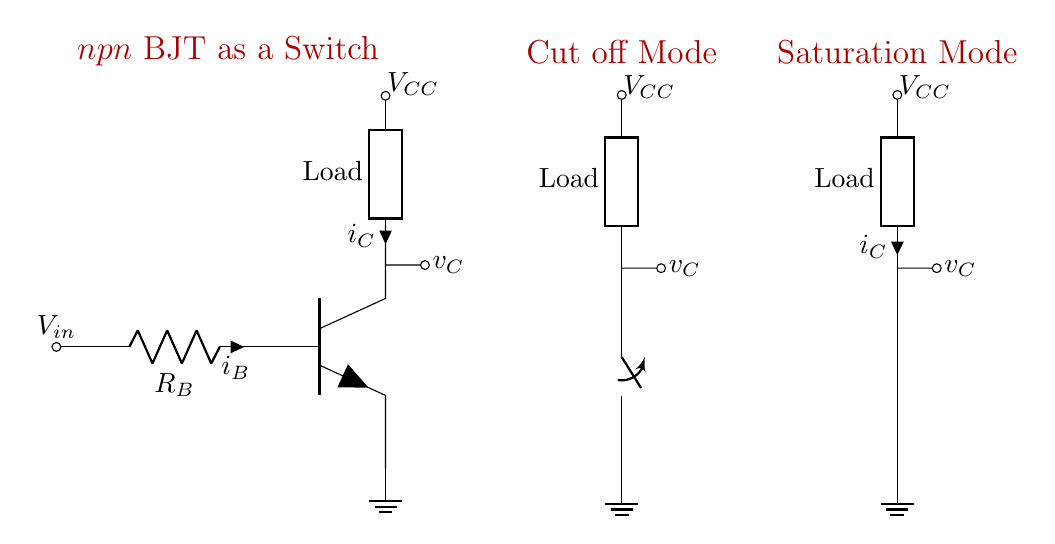
\begin{tikzpicture}
    \begin{scope}
        % Title
        \node[anchor=center, color=myred] at (-2, 3.75) {\large $npn$ BJT as a Switch};
        % npn BJT sumbol
        \draw (0, 0) node[npn, scale=2.0] (Q) {};
        \draw (Q.base) 
            to[R, R={$R_B$}, i<={$i_B$}] ++(-2.0, 0)
            to[short, -o, invert] ++(-0.5, 0);
        \node[anchor=center, align=center] at ($(Q.base) + (-2.5, 0.25)$) {$V_{in}$};
        \draw ($(Q.collector) + (0, -0.35)$)
            to[R, european, -o, R={Load}, i<={$i_C$}] ++(0, 2.0);
        \node[anchor=center, align=center] at ($(Q.collector) + (0.35, 1.8)$) {$V_{CC}$};
        \node[ground] at (Q.emitter) {};
        \draw ($(Q.collector) + (0, -0.5)$)
        to[short, -o] ++(0.5, 0);
        \node[anchor=center, align=center] at ($(Q.collector) + (0.8, -0.5)$){$v_{C}$};
    \end{scope}
    \begin{scope}[xshift=3cm]
        % Title
        \node[anchor=center, color=myred] at (0, 3.75) {\large Cut off Mode};
        % npn BJT sumbol
        \draw (0, 1.0)
        to[R, european, -o, R={Load}] ++(0, 2.2);
        \node[anchor=center, align=center] at (0.35, 3.3) {$V_{CC}$};
        \draw (0, 1.0)
            to[short, -o] ++(0.5, 0);
        % Open switch
        \draw (0, 1.0)
            to[ospst] ++(0, -2.75);
        \node[ground] at (0, -1.575) {};
        \node[anchor=center, align=center] at ($(0, 1.0) + (0.8, 0)$){$v_{C}$};
    \end{scope}
    \begin{scope}[xshift=6.5cm]
        % Title
        \node[anchor=center, color=myred] at (0, 3.75) {\large Saturation Mode};
        % npn BJT sumbol
        \draw (0, 1.0)
        to[R, european, -o, R={Load}, i<={$i_C$}] ++(0, 2.2);
        \node[anchor=center, align=center] at (0.35, 3.3) {$V_{CC}$};
        \draw (0, 1.0)
        to[short, -o] ++(0.5, 0);
        % Closed switch
        \draw (0, 1.0)
            to[short] ++(0, -2.75);
        \node[ground] at (0, -1.575) {};
        \node[anchor=center, align=center] at ($(0, 1.0) + (0.8, 0)$){$v_{C}$};
    \end{scope}
\end{tikzpicture}
\end{document}